\documentclass[a4paper, 12pt]{report}

% PACKAGES
% ------------------------------------------------------------------------
% INPUT
\usepackage[utf8]{inputenc}

% MARGINS
\usepackage{geometry}
\geometry{left=25mm, right=25mm, top=20mm, bottom=20mm}

% FOOTNOTE BELOW FIGURE
\usepackage[bottom, flushmargin]{footmisc}

% NAME REFERENCES
\usepackage{nameref}

% CUSTOM HEADER/FOOTER
\usepackage{fancyhdr}
\pagestyle{fancy}
\lhead{}
\chead{}
\rhead{}
\lfoot{Iteration \thechapter}
\cfoot{}
\rfoot{Page \thepage}
\renewcommand{\headrulewidth}{0pt}
\renewcommand{\footrulewidth}{0pt}

% MATH SYMBOLS
\usepackage{amsmath}
\usepackage{amssymb}

% HYPERLINKS
\usepackage{hyperref}
\hypersetup{colorlinks, linktocpage, linkcolor=black, urlcolor=black}

% GRAPHICS
\usepackage{graphicx}
\graphicspath{{images/}}

% CODE LISTING
\usepackage{listings}
\lstset{
    language=Python,
    basicstyle=\ttfamily\small,
    aboveskip={1.0\baselineskip},
    belowskip={1.0\baselineskip},
    belowcaptionskip=5mm,
    columns=fixed,
    extendedchars=true,
    breaklines=true,
    tabsize=4,
    prebreak=\raisebox{0ex}[0ex][0ex]{\ensuremath{\hookleftarrow}},
    frame=lines,
    framesep = 5mm,
    showtabs=false,
    showspaces=false,
    showstringspaces=false,
    keywordstyle=\color[rgb]{0.85,0.25,0.25}, % dark red
    commentstyle=\color[rgb]{0.5,0.5,0.5},    % mid grey
    stringstyle=\color[rgb]{0.85,0.65,0.10},  % dark yellow
    numbers=left,
    numberstyle=\small,
    stepnumber=1,
    numbersep=10pt,
    captionpos=t,
    escapeinside={\%*}{*)}
}

% PSEUDO CODE
\usepackage{algorithm2e}

% VERBATIM IN FOOTNOTES
\usepackage{fancyvrb}
\VerbatimFootnotes

% COMMANDS
% ------------------------------------------------------------------------
% horizontal line
\newcommand{\LINE}{\rule{\linewidth}{0.5pt}}
% tutor name
\newcommand{\tutor}{}
% make title
\makeatletter
\renewcommand{\maketitle}{
\vspace*{20pt}
\LINE\\
\vspace{2pt}\\
{\huge \noindent\sffamily{\@title}}\\
\vspace{2pt}\\
\hfill {\large \@date}\\
\vspace{2pt}\\
{\large \@author}\\
\vspace{2pt}\\
https://github.com/johnxnguyen/ElectionDB\\
\LINE\\
\vspace{4pt}
}
\makeatletter


% OTHER SETTINGS
% ------------------------------------------------------------------------

\linespread{1.3}
\setlength{\parindent}{0pt} % paragraph indentation
\setlength{\parskip}{10pt}  % space between paragraphs

% DOCUMENT
% ------------------------------------------------------------------------

\begin{document}

% TITLE
\title{\textbf{Database Systems}\\Project Documentation}
\date{02/06/2017}
\author{John Nguyen\\Gavithishan Ravechandran\\Khanh Bui Trong}
\maketitle
\thispagestyle{empty}

% ---------------------------------------------------------------
% ITERATION 1
% ---------------------------------------------------------------

\chapter{Project Iteration 1}
\label{ch:iteration1}

% SECTION 1: INTRODUCTION
% ---------------------------------------------------------------
\newpage
\section{Introduction}
\subsection{Project Aim}
The aim of this project to provide an interactive visualisation of tweet data collected prior to the american elections in 2016 from former presidential candidates Hillary Clinton and Donald J. Trump. It focuses primarily on the usage \emph{hashtags} and aims to facilitate a user-oriented analysis on these hashtags. This includes providing visualizations of relationships between hashtags regarding the frequency of their single and pairwise occurrences; the development of their usages over time; and their inherent importance\footnote{The importance of a hashtag is interpreted as the accumulative impact of the tweets that it belongs to.}. The final form of the project will be a web application that enables the user to interactively query the underlying database.

\subsection{Requirements}
The following list describes the type of requests that the web application must be able to respond to. Although this list is not exhaustive, the user should at least be able to retrieve the following information:
\begin{itemize}
  \item which hashtags were used, by whom and in which tweets
  \item how often a single hashtag, or a pair of hashtags, was used
  \item who used the most hashtags
  \item which hashtags were used the most
  \item in which period  hashtags (generally) used the most
  \item how did the usage of a hashtag (or pair) develop over time
  \item how the usage of a hashtag relates to the amount of times a tweet was retweet or favorited
\end{itemize}


\subsection{The Team}
This project is being developed by John Nguyen, Gavithishan Ravechandran and Khanh Bui Trong. We are all currently studying a Bachelor of Computer Science at the Freie Universität in Berlin, Germany.

% SECTION 2: DATA ANALYSIS
% ---------------------------------------------------------------
\newpage
\section{Data Analysis}
The data used in this project is a collation of tweet data produced by former american presidential candidates Hillary Clinton and Donald J. Trump prior to the 2016 election. The tweets were created between January and October and consist of the following components:
\begin{itemize}
  \item \texttt{handle:} indicates the user who posted the tweet
  \item \texttt{text:} the actual tweet content
  \item \texttt{is retweet:} indicates if the tweet is a retweet
  \item \texttt{original author:} indicates the original author of the tweet (applicable only to retweets)

  \item \texttt{time:} indicates the date and time the tweet was created
  \item \texttt{in reply to screen name:} if the tweet is a reply, this indicates who the reply is directed to

  \item \texttt{is quote status:} indicates if the tweet was quoted tweet
  \item \texttt{retweet count:} indicates the number of times the tweet was retweeted (by other users)

  \item \texttt{favorite count:} indicates how many times the tweet was favorited (by other users)

  \item \texttt{source url:} indicates from which platform (device) the tweet was published

  \item \texttt{truncated:} indicates if the tweet content was truncated
\end{itemize}

It is important note that not all components are necessarily relevant for the purposes of this project. For this reason the components \texttt{in reply to screen name}, \texttt{is quote status}, \texttt{source url} and \texttt{truncated} will be excluded from the data model (section 3).

For the remaining components we will briefly describe their importance: \texttt{handle, text} and \texttt{time} are core components that identify and describe particular tweet and the hashtags contained within; \texttt{favorite count} and \texttt{retweet count} describes the impact of the tweet; and finally \texttt{is retweet} and \texttt{original author} may provide additional contextual information about the tweet.

% SECTION 3: DATA MODEL
% ---------------------------------------------------------------
\newpage
\section{Data Model}
\subsection{The Entity-Relationship Model}
\label{sec:ermodel}

\begin{figure}[b]
  \centering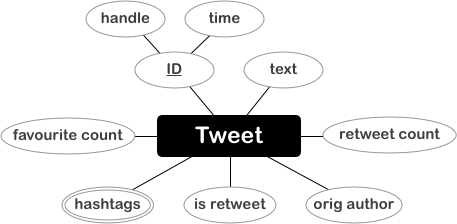
\includegraphics[scale = 0.8]{ERModel.png}
  \caption{The Entity-Relationship model of the dataset}
  \label{fig:ermodel}
\end{figure}

The Entity-Relationship model is depicted in Figure~\ref{fig:ermodel}. It consists of a single tweet-entity with a single value attribute for each component with the exception of \texttt{ID} and \texttt{hashtags}. Hashtags contained within the tweet text are represented as a multivalued attribute.

The key \texttt{ID} attribute is a composed from \texttt{handle} and \texttt{time}. The reason for this is because no single simple attribute forms a key since it can not be guaranteed that the value of this attribute will be distinct among multiple tweets objects. In other words, a pair of tweets may share a common value for each of the attributes. In order to uniquely identify a tweet, one must consider a combination of simple attributes. On the assumption that a single user may not publish two distinct tweets simultaneously, the paired value of \texttt{handle} and \texttt{time} forms a key\footnote{Although the time attribute is only precise to the second, the key remains valid in our (static) dataset.}.

A hashtag is not represented as an entity (nor their relationship to a tweet through a corresponding relationship type) because it increases unnecessary complexity to the model. A hashtag entity would have only a single attribute (to specify the hashtag name) and participate in a single relationship with the tweet entity. This is more simply expressed using the multivalued approach as in Figure~\ref{fig:ermodel}. One concern with the current model, however, is its capacity to express pairwise relationships between distinct hashtags. As we shall see in the next section, our ER-model does not limit us to fulfill this requirement, since its translation to the relational model expresses a hashtag as distinct relation\footnote{When discussing relational models, we will use the terms \emph{relation} and \emph{table} interchangeably.}.

\subsection{The Relational Model}
\label{sec:relationalmodel}

\begin{figure}[b]
  \centering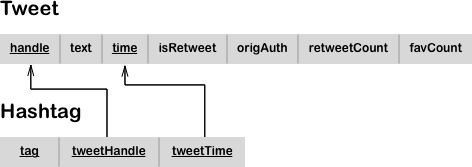
\includegraphics[scale = 0.8]{relationalModel.png}
  \caption{The relational model of the dataset}
  \label{fig:relationalmodel}
\end{figure}

The ER-model translates\footnote{The algorithm used is from: Fundamentals of Database Systems (7ED), Elmasri \& Navathe, 2016, ch. 9} into the relational model as illustrated in Figure~\ref{fig:relationalmodel}. It consists of two relations, one corresponding to the a tweet and the other to a hashtag. The primary key of the Tweet-relation is the tuple \texttt{(handle, time)}, as defined in section~\ref{sec:ermodel}.

The Hashtag-relation contains three attributes, the first of which, \texttt{tag}, stores the actual hashtag. The remaining two attributes \texttt{tweetHandle} and \texttt{tweetTime} form a foreign key referencing the primary key of the Tweet-relation. All three attributes then form the primary key of Hashtag-relation.

The following list specifies the domains and constraints of each attribute:

\subparagraph{handle:}
The domain is all alphanumeric (including underscores `\_') strings with maximum 15 characters\footnote{More specifically, this is any string matching the regular expression \verb+[a-zA-Z0-9_]{1,15}+.}. This attribute must have a value, i.e, it is constrained be \texttt{NOT NULL}, because it is part of the primary key. These constraints are defined by Twitter\footnote{See \verb+https://support.twitter.com/articles/101299#unavailable+}.

\subparagraph{text:}
The domain is all strings containing up to 140 characters. This attribute is constrained to be \texttt{NOT NULL}. These constrainst are also defined by Twitter\footnote{See \verb+https://support.twitter.com/articles/15367+}.

\subparagraph{time:}
The domain is all timestamps in the format \texttt{YYYY-MM-DD HH:MM:SS}. This attribute is constrained to be \texttt{NOT NULL} because it is part of the primary key.

\subparagraph{isRetweet:}
The domain is the set of boolean values $\{true, false\}$. This attribute is naturally constrained to be \texttt{NOT NULL}.

\subparagraph{origAuthor:}
The domain is the same as the \texttt{handle} attribute since it refers to another twitter user. The attribute will contain a value only if \texttt{isRetweet} set to true.

\subparagraph{retweetCount \& favCount:}
The domain is the set of positive whole numbers and the attribute is constrainted to be \texttt{NOT NULL}, since a tweet must be retweeted 0 or more times.

\subparagraph{tag:}
The domain is the set of all valid hashtags; strings containing alphanumeric characters (including underscores) but beginning with the \texttt{\#} symbol and otherwise containing at least one alphabetic letter. Because the entire tag is part of the tweet text, it may not exceed 140 characters in length\footnote{This is any string matching the regular expression \verb+#\w*[a-zA-Z]\w*'+.}. Due to this attribute being part of the primary key for the Hashtag-relation, it is constrained to be \texttt{NOT NULL}.

\subsection{Important Considerations}
\label{subsec:considerations}

The Hashtag-relation does not represent single hashtag objects, but rather the occurrences of hashtags. Thus each tuple in the Hashtag-relation pairs together the hashtag used, and the tweet it was used in.

Since the primary key of the Hashtag-relation is the set of the \texttt{tag}, \texttt{tweetHandle} and \texttt{tweetTime} attributes, each tuple within the relation must have a unique combination of values for these attributes. As a consequence, no single hashtag may occur multiple times in a single tweet because an attempt to insert two occurrences of the same hashtag from the same tweet leads to two tuples with equal attriubte values. This is a violation of the primary key constraint. To avoid this violation it is required that \textbf{the occurrence of a hashtag within a tweet is to be counted at most once}. This requirement does not adversely affect the goals of the projects since the functionality of a hashtag depends solely on its existence rather than its quantity.

% SECTION 4: CONSTRUCTING THE DATABASE
% ---------------------------------------------------------------
\newpage
\section{Constructing the Database}
\label{sec:constructingTheDatabase}

The database management system used in this project is \textit{PostgreSQL} (version 9.6). It can be installed by the \textit{Homebrew}\footnote{for macOS see https://brew.sh, or alternatively for linux see http://linuxbrew.sh. For instructions on installing PostgreSQL see \texttt{https://gist.github.com/sgnl/609557ebacd3378f3b72}.} package manager via the command line.

The PostgreSQL installation includes the command line application \texttt{psql}, with which we can execute the SQL statement required to create the database. Entering the command \texttt{psql} starts the application. Once inside \texttt{psql}, we can execute the following SQL statement:

\texttt{CREATE DATABASE election; }

This command creates a empty database called \texttt{election} based on the default settings. At this point in the project this is sufficient for experimentation purposes, however it may be necessary later to adjust the database settings to specify user access privileges and server information. We can confirm the database was created by entering the command:

\texttt{\textbackslash l}.

This lists all the exisitng databases. To quit \texttt{psql} simply enter the command:

\texttt{\textbackslash q}


% ---------------------------------------------------------------
% ITERATION 2
% ---------------------------------------------------------------

\chapter{Project Iteration 2}
\label{ch:iteration2}

% SECTION 1: SCHEMA
% ---------------------------------------------------------------
\newpage
\section{Database Schema}
Section ~\ref{sec:relationalmodel} outlines in detail the database schemas needed to be constructed. We must simply express the domains and constraints with SQL statements. Firstly we define two domains, \texttt{handle\_type} and \texttt{natural\_num}, which correspond to the set of all valid twitter handles and the set of all positive whole numbers. Note that PostgreSQL allows the use of \textit{regular expressions} within \texttt{CHECK} constraints, which we will utilize to validate the twitter handles. The following SQL statement defines the domains:

\begin{verbatim}
  CREATE DOMAIN HANDLE_TYPE AS VARCHAR(15) CHECK  (VALUE ~ '^\w{1,15}$');
  CREATE DOMAIN NATURAL_NUM AS INTEGER NOT NULL CHECK (VALUE >= 0);
\end{verbatim}

Next we define the schemas corresponding to the \textit{Tweets} and \textit{Hashtags} relations with the following SQL:

\begin{verbatim}
  CREATE TABLE Tweets (
        handle          HANDLE_TYPE     NOT NULL,
        content         VARCHAR(140)    NOT NULL,
        t_stamp         TIMESTAMP       NOT NULL,
        is_retweet      BOOLEAN         NOT NULL,
        orig_author     HANDLE_TYPE,
        retweet_count   NATURAL_NUM,
        fav_count       NATURAL_NUM,
        PRIMARY KEY (handle, t_stamp)
    );

    CREATE TABLE Hashtags (
          tag           VARCHAR(140)  NOT NULL
          CHECK (tag ~ '^#\w*[a-zA-Z]\w*$'),
          tweet_handle  HANDLE_TYPE   NOT NULL,
          tweet_t_stamp TIMESTAMP     NOT NULL,
          PRIMARY KEY (tag, tweet_handle, tweet_t_stamp),
          FOREIGN KEY (tweet_handle, tweet_t_stamp)
          REFERENCES Tweets(handle, t_stamp)
          ON UPDATE CASCADE ON DELETE CASCADE
      );
\end{verbatim}

We note that if a tweet is updated or deleted from the Tweets relation, then any hashtags from the Hashtag relation that references this tweet will also be updated or deleted.

The Python script in listing~\ref{lst:tableCreator} creates the relation schemas by first connecting to the \texttt{election} databse and then sequentially executing each of the SQL statements above. Note that before the domains and tables are created, the script first checks to see if they exist, and if so, they are deleted. This allows the program to be run even if the database is not empty and is included as a convenience. The \textit{psycopg2} Python package is used to communicate with PostgreSQL.

\lstinputlisting[language = python, caption = table\_creator.py]{../../Code/DBBuilder/table_creator.py}
\label{lst:tableCreator}

% DATA CLEANING
% ----------------------------------------------------------------------
\newpage
\section{Data Cleaning}
\label{sec:dataCleaning}
In order to correctly import the data into the database, we must first prepare and clean the raw data. This involves extracting only the necessary data, formatting the data components into the expected data types as defined by the corresponding relation schema, as well as removing or correcting any other anomalies.

Of all the attributes listed in the schemas of the previous section, only \texttt{content} and \texttt{t\_stamp} attributes need to be reformatted.

\subparagraph{content:} In the raw data file, some tweet entries contain symbols encoded for web usages. These include \texttt{\&}, \texttt{<}, and \texttt{>}, and appear in the raw data as \texttt{\&amp;}, \texttt{\&lt;}, and \texttt{\&gt;} respectively. Thus we must replace each occurrence of these encoded symbols with the decoded symbols they represent.

\subparagraph{t\_stamp:} In the raw data file, this element has the form \texttt{yyyy-mm-ddThh:mm:ss}; for example \texttt{2017-01-01T00:00:00} represents midnight on the 1st of January 2017. However, the \texttt{TIMESTAMP} data type in PostgreSQL is expected to be in the form \texttt{yyyy-mm-dd~ hh:mm:ss}; the only difference is absence of the letter \texttt{T}. Therefore we must replace the letter \texttt{T} with a space for every entry of this data element in the raw data.

All the other data elements corresponding to the remaining attributes are already in the appropriate format and thus no additional conversions are required.

The Python script shown in listing~\ref{lst:dataCleaner} automates this process by reading the raw data, performing the conversions, and writing only the needed (and cleaned) data into a new file. The raw data has been provided in two different file formats: \texttt{xlsx} (excel spreadsheet) and \texttt{csv} (comma separated values). We have chosen to work with the \texttt{xlsx} file because it is better structured compare to the \textit{csv} file. Each line of \texttt{csv} file does not always represent a complete tweet entry; multiline tweets (those with newline characters) are spread across multiple lines within the \texttt{csv} file and thus pose a problem when trying to parse this file.

This problem does not arise when parsing a spreadsheet; all tweet elements are contained within individual cells, including multiline tweets. Thus the program can easily iterate through each row and then through each cell to extract the elements accordingly. Furthermore, the standard Python \texttt{csv} parsing module does not support unicode strings (and therefore also the emojis contained in the tweets), whereas the spreadsheet does. The program utilizes the \textit{openpyxl} package for reading and writing the \texttt{xlsx} file format.

\lstinputlisting[language = python, caption = data\_cleaner.py]{../../Code/DBBuilder/data_cleaner.py}
\label{lst:dataCleaner}

% IMPORTING THE DATA
% ----------------------------------------------------------------------
\newpage
\section{Importing the data}
\label{sec:dataImporting}

The Python script in listing~\ref{lst:tablePopulator} automates the insertion of the cleaned data into the database. It first makes a connection to the database, then iterates through each row of the data file (\texttt{xlsx} format) and inserts both the tweet data and the hashtag data contained in this row. The structure of the data file corresponds to the \texttt{Tweets} table and thus we can simply insert the whole row directly into this table. The hashtag data must be extracted from the current tweet content, which is achieved by using a regular expression to find any embedded hashtags. As noted in section~\ref{subsec:considerations}, only distinct hashtags are extracted. Once a list of distinct hashtags is obtained, the program then inserts a new row into the \texttt{Hashtags} table for each hashtag with a reference to the current tweet.

Finally, the insertions are committed to the database and the number of insertions is reported back to the user.

\lstinputlisting[language = python, caption = table\_populator.py]{../../Code/DBBuilder/table_populator.py}
\label{lst:tablePopulator}

% EXECUTING THE CODE
% ----------------------------------------------------------------------
\newpage
\section{Executing the code}

For simplicity, the code presented in the previous three sections have been collated into a sinlge Python script called \texttt{dbBuilder.py}. Running this script within terminal from the working directory will clean the raw data, save it to a new file, connect to the database, create the schemas and finally import the cleaned data. It is assumed the database \texttt{election} already exists and is configured, however it is not required that the database is empty because the program will drop all schemas before recreating them.

The database name, username, and password are stored in the \texttt{config.py} file, which is used to establish the connection to PostgreSQL. These parameters must match the configuration of the local machine in order for the connection to be successful.

% WEB SERVER
% ----------------------------------------------------------------------
\section{Web Server}
We have chosen to use the open source server software \texttt{Apache}, which is included in the \textit{macOS Sierra} operating system. It is configured at both the system wide level and the user level. The server root directory on the system level is located at:

\begin{verbatim}
  /Library/WebServer/Documents
\end{verbatim}

and can be accessed in the web browers at the url:

\begin{verbatim}
  http://localhost
\end{verbatim}

The server root directory on the user level is located at:

\begin{verbatim}
  ~/Sites
\end{verbatim}

and can be accessed in the web browers at the url:

\begin{verbatim}
  http://localhost/~username
\end{verbatim}

where \texttt{username} is a placeholder for the username of on the local machine.


\end{document}
